\documentclass{beamer}
\usepackage[utf8]{inputenc}
\usepackage[spanish]{babel}
\usepackage{multicol}
\decimalpoint
\usetheme{Antibes}
\usecolortheme{seahorse}
\setbeamertemplate{bibliography item}{\insertbiblabel}
\begin{document}
\title{Avance de trabajo de Tesis.}
\author{David Gustavo Merinos Sosa}
\date{\today}

\frame{\titlepage}
\section{Datos de la tesis.}

\frame{
\begin{block}{Datos de la tesis.}
  \begin{itemize}
    \item Nombre: Descomposición de gráficas geométricas completas en thrackles: un enfoque computacional para conjuntos con hasta diez puntos.
    \item Directora: Dra. María Dolores Lara Cuevas
    \item Área: Geometría combinatoria, geometría computacional.
  \end{itemize}
  \end{block}
}
\section{Antecedentes}
\frame{\frametitle{Algunas definiciones}
\begin{block}{Gráfica completa de $n$ vértices. ($K_n$)}
  Una gráfica es completa cuando existe una arista entre cada par de vértices. La gráfica completa de $n$ vértices tiene
  $\binom{n}{2}$ aristas.
  \begin{figure}[h]
    \caption{De izquierda a derecha se muestran gráficas completas de 3, 4 y 5 vértices respectivamente}
    \centering
    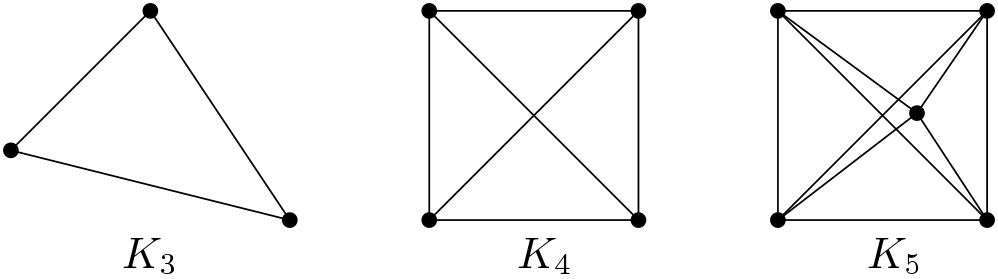
\includegraphics[width=8cm]{imagenes/knex.png}
  \end{figure}
  \end{block}
}
\frame{\frametitle{Algunas definiciones}
\begin{block}{Gráfica geométrica}
  Es la representación de una gráfica en el plano, donde cada vértice es representado por un punto en el plano y cada arista
  es representada por un segmento de recta que une dos puntos.\\[2mm]

  \begin{figure}[h]
    \caption{$K_4$ y gráficas geométricas de $K_4$ distintos.}
    \centering
    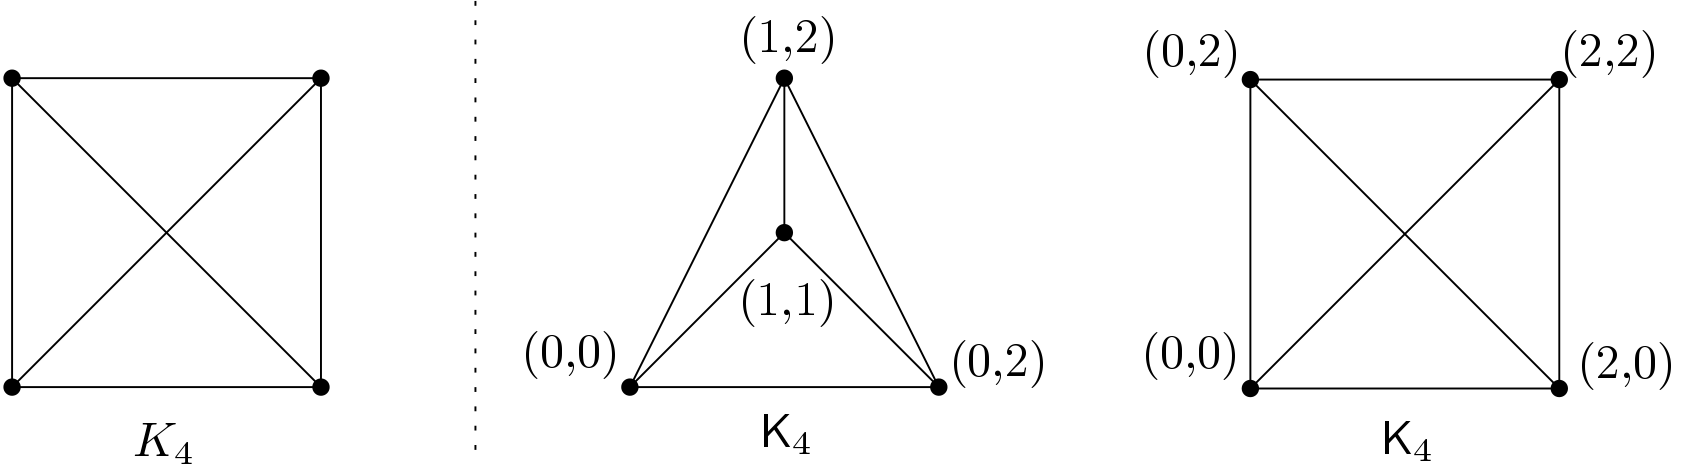
\includegraphics[width=9cm]{imagenes/drawings.png}
  \end{figure}
\end{block}
}
\frame{\frametitle{Algunas definiciones}
  \begin{block}{Descomposición de una gráfica.}
    Una descomposición de una gráfica $G$ es una colección $D=\{G_1,G_2,\dots,G_k\}$ de subgráficas de $G$ tal que se cumplan:
    \begin{enumerate}
      \item Ninguna subgráfica $G_i$ tiene vértices aislados.
      \item Cada arista de $G$ pertenece a exactamente un elemento de $D$.
    \end{enumerate}
  \end{block}
}

\frame{\frametitle{Algunas definiciones}
  \begin{block}{Thrackle.}
    Un thrackle es una gráfica geométrica en la que cada par de aristas se intersecta. \\[2mm] Un thrackle en un conjunto de $n$ vértices es máximo si tiene $n$ aristas.
    \begin{figure}[h]
      \caption{Ejemplo de un thrackle de 5 vértices.}
      \centering
      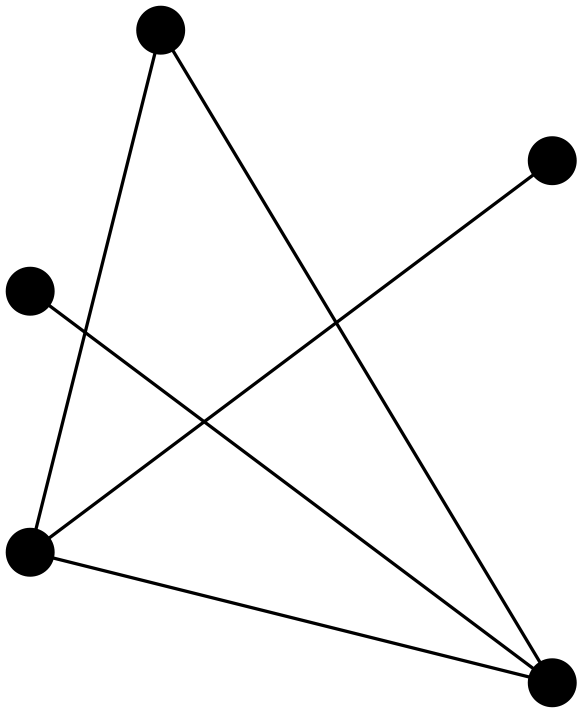
\includegraphics[width=2.4cm]{imagenes/thrackle.png}
    \end{figure}
  \end{block}
}

\frame{\frametitle{Algunas definiciones}
  \begin{block}{Anti-thickness de una gráfica geométrica}
    El anti-thickness de una gráfica geométrica $\mathsf{G}$ es la $k$ más pequeña tal que se puede dar una descomposición
    de las aristas de $\mathsf{G}$ en $k$ thrackles.
  \end{block}
  \begin{block}{Anti-thickness geométrico}
    El anti-thickness geométrico de una gráfica $G$, $\mathsf{at_g}(G)$ es la $k$ más pequeña tal que $G$ tiene un gráfica geométrica con anti-thickness $k$.
  \end{block}
}
\section{Descomponiendo $K_9$}
\frame{\frametitle{El anti-thickness geométrico de $K_9$ es 6.}
\begin{block}{Es equivalente decir...}
  Existe una gráfica geométrica de $K_9$ que puede ser descompuesta en 6 thrackles y además no existe ningúna gráfica geométrica de $K_9$ que pueda ser descompuesta con menos de 6 thrackles.
\end{block}
}
\frame{\frametitle{El anti-thickness geométrico de $K_9$ es 6.}
\begin{block}{Mejorando las cotas.}
  De la literatura sabemos que $\mathsf{at_g}(K_n) \in [\frac{n-1}{2},n - \lfloor \sqrt{2n + \frac{1}{4}} - \frac{1}{2}\rfloor]$
\end{block}
}

\frame{\frametitle{El anti-thickness geométrico de $K_9$ es 6.}
\begin{block}{Mejorando las cotas.}
  \[\mathsf{at_g}(K_n) \in [\frac{n-1}{2},n - \lfloor \sqrt{2n + \frac{1}{4}} - \frac{1}{2}\rfloor]\]
  Para $n=9$ :
  \[\mathsf{at_g}(K_9) \in [\frac{9-1}{2},9 - \lfloor \sqrt{2(9) + \frac{1}{4}} - \frac{1}{2}\rfloor]\]
  \[\mathsf{at_g}(K_9) \in [4,6]\]
\end{block}
}
\frame{}

\frame{\frametitle{El anti-thickness geométrico de $K_9$ es 6.}
\begin{block}{Buscando una descomposición de tamaño 5.}
  Es necesario analizar todas las descomposiciones de tamaño 5 o menos para 36 aristas.
  \begin{multicols}{2}
  \begin{itemize}
    \item 9 + 8 + 8 + 8 + 3
    \item 9 + 8 + 8 + 7 + 4
    \item 9 + 8 + 8 + 6 + 5
    \item 9 + 8 + 7 + 7 + 5
    \item 9 + 8 + 7 + 6 + 6
    \item 9 + 7 + 7 + 7 + 6
    \item 8 + 8 + 8 + 8 + 4
    \item 8 + 8 + 8 + 7 + 5
    \item 8 + 8 + 8 + 6 + 6
    \item 8 + 8 + 7 + 7 + 6
    \item 8 + 7 + 7 + 7 + 7
  \end{itemize}
  \end{multicols}
\end{block}
}
\frame{\frametitle{El anti-thickness geométrico de $K_9$ es 6}
\begin{block}{Analizando una descomposición.}
  Al analizar una descomposición, por ejemplo: 9 + 7 + 7 + 7 + 6, necesitamos verificar todos los thrackles
  de tamaño 9, todos los thrackles de tamaño 7 y todos los thrackles de tamaño 6.
\end{block}
}
\frame{\frametitle{El anti-thickness geométrico de $K_9$ es 6}
\begin{block}{Analizando una descomposición.}
  Para hacerlo, usamos un algoritmo de back-tracking que agrega thrackles a la descomposición cuando las aristas son
  totalmente disjuntas. Esto es, agrega un thrackle de tamaño 9 y uno de 7 si no comparten aristas, repetimos esto para cada
  elemento de la descomposición 9 + 7 + 7 + 7 + 6.
\end{block}
}
\frame{\frametitle{El anti-thickness geométrico de $K_9$ es 6}
\begin{block}{Descomposición válida}
 Una descomposición de la forma 9 + 7 + 7 + 7 + 6, es válida si existen 5 thrackles, uno de tamaño 9, tres de tamaño 7 y uno de tamaño 6 que no compartan aristas a pares.
\end{block}
}

\frame{\frametitle{El anti-thickness geométrico de $K_9$ es mayor a 5}
\begin{block}{Resultados}
 Después de analizar todas las posibles descomposiciones, no fue posible encontrar una que fuera válida. Esto puede traducirse en que ninguna de las descomposiciones en thrackles cubría las 36 aristas necesarias, lo que a su vez significa que se necesitan más de 5 thrackles para cubrir la gráfica completa.
 \[\mathsf{at_g}(K_9) > 5\]
 \[\mathsf{at_g}(K_9) \in (5,6]\]
 \[\mathsf{at_g}(K_9) = 6\]
\end{block}
}

\frame{
  \centering \Large
  \emph{Fin,¿preguntas?}
}
\section{Extra}
\frame{
  \begin{block}{Analizar todos los dibujos geométricos de $K_n$}
    Hay un número infinito de dibujos geométricos para cualquier conjunto de puntos en el plano.
    Para analizarlos todos usamos el tipo de orden que es una forma de clasificar los dibujos geométricos
    de acuerdo a sus propiedades combinatorias.
    \begin{table}
      \centering
      \begin{tabular}{c|c}
        $n$ & No. tipos de orden \\
        3 & 1 \\
        4 & 2 \\
        5 & 3 \\
        6 & 16 \\
        7 & 135 \\
        8 & 3315 \\
        9 & 158817 \\
        10 & 14309547
      \end{tabular}
    \end{table}
  \end{block}
}
\frame{
\begin{block}{Tiempos de ejecución}
  Para cada uno de las decomposiciones se almacenaron los tiempos de ejecución.
    \begin{multicols}{2}
  \begin{itemize}
    \item 9 + 8 + 8 + 8 + 3 -
    \item 9 + 8 + 8 + 7 + 4 -
    \item 9 + 8 + 8 + 6 + 5 -
    \item 9 + 8 + 7 + 7 + 5 - 16 minutos.
    \item 9 + 8 + 7 + 6 + 6 - 16 minutos.
    \item 9 + 7 + 7 + 7 + 6 - 35 minutos.
    \item 8 + 8 + 8 + 8 + 4 - 5 minutos.
    \item 8 + 8 + 8 + 7 + 5 - 9 minutos.
    \item 8 + 8 + 8 + 6 + 6 - 9 minutos.
    \item 8 + 8 + 7 + 7 + 6 - 1 Hora, 46 minutos.
    \item 8 + 7 + 7 + 7 + 7 - 34 Horas, 21 minutos.
  \end{itemize}
\end{multicols}
\end{block}
}
\end{document}
